%% USE one of these:
%% * the first when using pdflatex, which directly typesets your document in the
%%   chosen pdf/a format and you want to publish your thesis online,

%% * the second when you want to print your thesis to bind it, or
%% * the third when producing a ps file and a pdf/a from it.
%%
\documentclass[english, 12pt, a4paper, elec, utf8, a-1b, online]{aaltothesis}
%\documentclass[english, 12pt, a4paper, elec, utf8, a-1b]{aaltothesis}
%\documentclass[english, 12pt, a4paper, elec, dvips, online]{aaltothesis}


\UseRawInputEncoding
\usepackage{graphicx}
\usepackage{amsfonts,amssymb,amsbsy,amsmath, enumitem, siunitx, array}
\usepackage{float}
\usepackage[justification=centering]{caption}

\graphicspath{ {./images/} }

%% THESIS INFO
\degreeprogram{Electrical engineering}

\major{Bioinformation technology}

\code{ELEC3016}

\univdegree{BSc}

\thesisauthor{Axel Hedman}

\thesistitle{Fasting Plasma Glucose Assessed by Continuous Glucose Monitoring}

\place{Espoo}

\date{4.5.2023}

\supervisor{PhD\ Markus Turunen}

\advisor{D.Sc\ Lauri Palva}
\advisor{Mgr.\ Matej Kr\'{a}lik}


%% Aaltologo: syntax:
%% \uselogo{aaltoRed|aaltoBlue|aaltoYellow|aaltoGray|aaltoGrayScale}{?|!|''}
\uselogo{aaltoRed}{!}


%% THE ENGLISH ABSTRACT:
%% Thesis keywords:
\keywords{continuous glucose monitoring\spc metabolic health\spc fasting plasma glucose}

%% The abstract text. This text is included in the metadata of the pdf file as well
%% as the abstract page.

\thesisabstract{
The prevalence of obesity and overweight is a growing health issue worldwide. Obesity 
increases the risk for metabolic complications including 
diabetes mellitus, cardiovascular disease, and various types of cancer. 
An unhealthy lifestyle is a leading cause of obesity. Lifestyle changes have been proven an effective approach to overcoming obesity and overweight. 
Fasting plasma glucose (FPG) is an established indicator of whether 
an individual is metabolically healthy. Traditionally an FPG test requires
a medical appointment including  a blood sample. Such a test requires the user to fast for at least 8 hours before measuring FPG levels from a blood sample.
Newer research has challenged the need for an 8-hour fasting widow and suggests that FPG levels may be achieved by a shorter fasting period. Modern technology has brought alternative solutions to 
blood glucose monitoring. Today, continuous glucose monitoring (CGM) devices can be paired with smartphones and utilize mobile applications
to streamline the glucose monitoring process.
This thesis explores the possible usage of CGM data to approximate FPG. The continuous stream of glucose data 
provided by a CGM device and meal information allows for thorough glucose analysis. Regular FPG approximations can 
be utilized to optimize lifestyle for maintaining good metabolic health. 
The thesis investigates and demonstrates possible methods for approximating FPG. The demonstrations presented in this thesis are made possible by a collaboration with a company named Veri.
The CGM data and event information used in this thesis is provided by Veri. The demonstrations are mainly visual and illustrate how FPG can be approximated from CGM data. The visual demonstrations compare an 8-hour fasting window with a shorter fasting window of 3 hours. This thesis's main contribution to the field is that FPG approximations based on CGM data are possible. 
}

%% Copyright text. Copyright of a work is with the creator/author of the work
%% regardless of whether the copyright mark is explicitly in the work or not.
%% You may, if you wish, publish your work under a Creative Commons license (see
%% creaticecommons.org), in which case the license text must be visible in the
%% work. Write here the copyright text you want. It is written into the metadata
%% of the pdf file as well.
%% Syntax:
%% \copyrigthtext{metadata text}{text visible on the page}

\copyrighttext{Copyright \noexpand\copyright\ \number\year\ \ThesisAuthor}
{Copyright \copyright{} \number\year{} \ThesisAuthor}


\begin{document}

%% Create the coverpage
\makecoverpage


%% Typeset the copyright text.
%% If you wish, you may leave out the copyright text from the human-readable
%% page of the pdf file. This may seem like a attractive idea for the printed
%% document especially if "Copyright (c) yyyy Eddie Engineer" is the only text
%% on the page. However, the recommendation is to print this copyright text.
\makecopyrightpage


%% ENGLISH ABSTRACT
%% All the details (name, title, etc.) on the abstract page appear as specified
%% above.
\pagenumbering{gobble}
\begin{abstractpage}[english]
    \abstracttext{}
\end{abstractpage}

%% Force a new page so that the Swedish abstract starts from a new page
\newpage

%% SWEDISH ABSTRACT.
\thesistitle{Fasteplasmaglukos fastst\"{a}llt av kontinuerlig glukosmonitorering}
\supervisor{PhD\ Markus Turunen}
\advisor{TkD\ Lauri Palva} 
\advisor{Mgr. Matej Kr\'{a}lik} 
\degreeprogram{Elektroteknik}
\major{Bioinformationsteknologi}
\keywords{metabol h\"{a}lsa\spc kontinuerlig glukosmonitorering\spc fasteplasmaglukos}
\begin{abstractpage}[swedish]
F\"{o}rekomsten av fetma och \"{o}vervikt \"{a}r ett v\"{a}xande h\"{a}lsoproblem v\"{a}rlden \"{o}ver. Idag \"{a}r n\"{a}rmare en tredjedel av v\"{a}rldens befolkning antingen \"{o}verviktiga eller diagnostiserade med fetma. Fetma \"{o}kar risken f\"{o}r en rad metabola komplikationer inklusive diabetes mellitus, kardiovaskul\"{a}ra sjukdomar och diverse cancerformer. En oh\"{a}lsosam livsstil har visat sig vara en av de ledande orsakerna till fetma. N\"{a}ringsintag, s\"{o}mn, stress och tr\"{a}ning p\aa verkar alla kroppens blodsockerniv\aa er. F\"{o}r att uppr\"{a}tth\aa lla h\"{a}lsosamma blodsockerniv\aa er kr\"{a}vs gynnsam f\"{o}rvaltning av alla livsstilsrelaterade delomr\aa den.
Fasteplasmaglukos \"{a}r en etablerad indikator n\"{a}r det kommer till metabol h\"{a}lsa. F\"{o}r att m\"{a}ta fasteplasmaglukos kr\"{a}vs en fasteperiod av f\"{o}rbest\"{a}md varaktighet. Under fasteperioden b\"{o}r patienten avst\aa\ fr\aa n alla former av kaloriintag. Ett fasteplasmaglukostest har traditionellt kr\"{a}vt ett l\"{a}karbes\"{o}k med ett tillh\"{o}rande blodprov. Modern teknologi har tillf\"{o}rt alternativa metoder till blodsockerm\"{a}tning. Kontinuerlig glukosmonitorering har visat sig vara ett konkurrenskraftigt alternativ till blodsockerm\"{a}tning. Idag kan mobila applikationer kombineras med kontinuerlig glukosmonitorering f\"{o}r att f\"{o}rse anv\"{a}ndaren med kontinuerliga glukosdata direkt i smarttelefonen. 
Detta arbete utforskar m\"{o}jligheten att approximera fasteplasmaglukos med hj\"{a}lp av kontinuerlig glukosmonitorering. Approximering av fasteplasmaglukos kr\"{a}ver s\aa v\"{a}l glukosdata som information ang\aa ende n\"{a}ringsintag. Den kontinuerliga datastr\"{o}mmen tillhandah\aa llen av kontinuerlig glukosmonitorering tillsammans med information ang\aa ende n\"{a}ringsintag till\aa ter genomg\aa ende blodsockeranalys. Regelbundna approximationer av fasteplasmaglukos kan anv\"{a}ndas f\"{o}r att uppr\"{a}tth\aa lla en h\"{a}lsosam livsstil och f\"{o}rebygga metabol sjukdom. F\"{o}rh\"{o}jda fasteplasmaglukosniv\aa er under en l\"{a}ngre tidsperiod indikerar att \aa tg\"{a}rder b\"{o}r vidtas f\"{o}r att f\"{o}rhindra sjukdom. Med regelbundna approximationer av fasteplasmaglukos kan patienten sj\"{a}lv f\"{o}lja med och reagera p\aa\ onormala fasteplasmaglukostrender. F\"{o}r\"{a}ndringar i livsstil kan s\"{a}nka fasteplasmaglukos. Om livsstilsf\"{o}r\"{a}ndringar inte hj\"{a}lper \"{a}r den rekommenderade \aa tg\"{a}rden att s\"{o}ka professionell hj\"{a}lp. 
Arbetets slutsats \"{a}r att approximation av fasteplasmaglukos med hj\"{a}lp av kontinuerlig glukosmonitorering \"{a}r m\"{o}jlig. Fasteplasmaglukosapproximaitoner kr\"{a}ver information ang\aa ende n\"{a}ringsintag. F\"{o}r att framg\aa ngsrikt approximera fasteplasmaglukos b\"{o}r fasteperioden tas i beaktande. Ytterligare forskning kr\"{a}vs f\"{o}r att fastst\"{a}lla den mest exakta metoden f\"{o}r approximation av fasteplasmaglukos med hj\"{a}lp av kontinuerlig glukosmonitorering. 
\end{abstractpage}

%% PREFACE
%% This section is optional.
%%\vspace{5mm}
%%{\hfill Axel J.\ H.\ Hedman \hspace{1cm}}

%%\newpage


%% TABLE OF CONTENTS
\thesistableofcontents


%% SYMBOLS AND ABBREVIATIONS
\mysection{Abbreviations}

\subsection*{Abbreviations}

\begin{tabular}{ll}
BMI         & body mass index \\
CGM      & continuous glucose monitoring \\
FPG        & fasting plasma glucose \\
IFG         & impaired fasting glucose \\
IGT         & impaired glucose tolerance \\
MARD        &  mean absolute relative difference \\
OGTT        & oral glucose tolerance test \\
\end{tabular}

\cleardoublepage

%% List of research questions
\newlist{questions}{enumerate}{2}
\setlist[questions,1]{label=RQ\arabic*.,ref=RQ\arabic*}
\setlist[questions,2]{label=(\alph*),ref=\thequestionsi(\alph*)}


%%%%%%%%%%%%%%%%%%
%% INTRODUCTION %%
%%%%%%%%%%%%%%%%%%
\pagenumbering{arabic}
\section{Introduction}
\thispagestyle{empty}

%% TEXT %%
A growing health issue worldwide is the prevalence of obesity and overweight. Since 1980, the number of patients 
diagnosed with obesity and overweight has doubled. Today, nearly a third of 
the world's population is considered obese or overweight 
\cite{chooi_epidemiology_2019}. As the prevalence of obesity and overweight 
increases, public health is at risk. Obesity affects 
nearly all physiological activity in the human body. It 
lowers life expectancy and increases the risk of multiple 
severe diseases including diabetes mellitus, 
cardiovascular disease, and various types of cancer\cite{chooi_epidemiology_2019}\cite{nammi_obesity_2004}. 
There are several approaches on how to tackle obesity and 
overweight but the majority of them revolve around 
diet and lifestyle management. Medications and surgery may solve 
short-term complications but several studies have shown 
that lifestyle changes are necessary to ultimately 
overcome obesity\cite{nammi_obesity_2004}\cite{mauro_barriers_2008}\cite{powell_effective_2007}.

Traditionally, glucose levels have been monitored with blood 
samples and finger pricks. When used correctly, glucose monitoring can be a useful tool when tracking 
changes in patients' lifestyles. Sleep, Diet, stress, and exercise affect blood
glucose levels as well as overall health\cite{yamaoka_effects_2012}. Studies have shown that correctly applied lifestyle changes
not only lower blood glucose levels but they also result in a lower body mass index (BMI) and weight,
improved cholesterol and triglyceride values, and lower blood pressure\cite{yamaoka_effects_2012}.
If not managed correctly, blood glucose levels can reach unusually high or low levels potentially causing 
acute and chronic conditions\cite{mathew_blood_2022}.  

A combination of obesity
and unnecessarily high glucose levels can lead to the onset of type 2 diabetes\cite{garber_obesity_2012}.
Type 2 diabetes patients are heavily dependent on glucose monitoring 
to correctly use medications and avoid critical conditions\cite{ripsin_management_2009}. 
Nevertheless, studies have shown that
with appropriate lifestyle changes, type 2 diabetes can be reversed with diet alone\cite{taylor_type_2013}. 
Such a reversal requires a fundamental understanding of how diet affects blood glucose.
Hence, glucose management and monitoring is a vital part of alleviating and 
preventing obesity and type 2 diabetes.

Fasting plasma glucose (FPG) is an established indicator of whether 
an individual is metabolically healthy or not\cite{moebus_impact_2011}\cite{danaei_national_2011}. 
FPG is usually measured from a blood sample taken after a minimum of 8 
hours of fasting\cite{the_expert_committee_on_the_diagnosis_and_classification_of_diabetes_mellitus_report_1997}. 
An FPG test traditionally requires a medical appointment. Before attending the medical appointment, patients 
have to go through the 8-hour fasting window. A procedure that may be perceived as disruptive. 

Modern technology has brought alternative glucose measurement methods. 
Continuous glucose monitoring (CGM) is an already introduced method to 
monitor blood glucose\cite{danne_international_2017}. CGM 
has struggled to become a medically approved method due to
large measurement errors - because in the year 2000, the mean absolute relative difference
(MARD) of CGM was larger than $\pm$20\% which is the accepted average for 
regulatory approval. As technology is advancing the MARD of CGM has 
now reduced to under $\pm$10\% and the accuracy continues to improve\cite{rodbard_continuous_2016}\cite{gifford_cgm}.

CGM uses an invasive electrochemical biosensor to measure glucose levels
in the interstitial fluid between cells.
The biosensor utilizes a small filament inserted through the skin 
to measure glucose levels. The in vivo response to a needle-type 
biosensor has been one of the biggest challenges to accurate CGM
measurements. The infiltration of proteins, the release of cytokines 
and reactive oxygen species, and subsequent influx of 
inflammatory cells all contribute to the instability of implanted 
glucose sensors.\cite{gifford_cgm}. Nevertheless, compared to
blood samples and finger pricks, CGM provides a complete set 
of continuous glucose data for the user to analyze. A finger
prick, for example, doesn't provide an overview of the long-term
effects that lifestyle and diet have on glucose levels. Hence, CGM
has established itself as a viable option when it comes to 
glycemic control and overall improvement of metabolic health. 

This thesis is done in collaboration 
with Veri\cite{noauthor_veri_nodate}, a Finnish company focusing on improving 
metabolic health through CGM. Veri combines a mobile application with a CGM 
sensor providing continuous glucose data for the user to analyze. By tracking 
glucose levels with CGM, users are able to observe the metabolic impact
of diet, sleep, stress, exercise, and other lifestyle factors on long-term health. 
To support the research and conclusions of this thesis, Veri has 
provided deidentified glucose data to help visualize trends in blood glucose. The provided data set
includes meal, exercise, sensor, and demographic data. 

This thesis aims to explore the possibility of using CGM 
data to approximate FPG by comparing a traditional 8-hour fasting window to a shorter fasting window of 3 hours.
By utilizing the continuous data stream of a CGM device, FPG approximations can be made based 
on large portions of data compared to the momentary blood sample of a traditional FPG test\cite{the_expert_committee_on_the_diagnosis_and_classification_of_diabetes_mellitus_report_1997}.
 
The advantage of FPG approximations assessed by CGM is how they can be continuously acquired 
from day to day without having to schedule a doctor's appointment. Likewise, the approximation includes data 
acquired over a longer period of time compared to the momentary blood sample of a traditional FPG test. 
Earlier research on the topic and visual demonstrations using the data provided by Veri will
be the supporting pillars when examining the possibility of approximating FPG from CGM data. 


Chapter 2 describes the background including central concepts connected to the topic. In Chapter 3, the data used to illustrate
glucose trends is presented. Chapter 4 demonstrates the possibilities of how FPG can be approximated from CGM data and discusses 
possible use cases. Chapter 5 further discusses the possible methods presented in Chapter 4 and Chapter 6 concludes the thesis. 
%% END TEXT %%
\clearpage


%%%%%%%%%%%%%%%%
%% BACKGROUND %%
%%%%%%%%%%%%%%%%
\section{Background}
%% TEXT %%
This chapter defines fundamental concepts and methods closely related to the topic 
of this thesis. The physiology behind glucose absorption is explained as well as interstitial glucose and fasting plasma glucose (FPG). The chapter also discusses how 
lifestyle has an impact on blood glucose and how elevated FPG levels can lead to health-related complications. 
Continuous glucose monitoring (CGM) is described as it is the method used to obtain the glucose data used in this thesis.

\subsection{Glucose absorption}
Glucose is one of the primary energy sources of the human body. It is a monosaccharide composed of Carbon, Hydrogen, and Oxygen. During digestion, carbohydrates are broken down into monosaccharides including glucose. Glucose is absorbed into the bloodstream by the small intestine\cite{glucose_absorption}. 

A family of G-protein coupled receptors, known as sweet taste receptors, located in the 
small intestine are responsible for glucose detection and absorption. Together with glucose transporters, including SGLT1 and 
GLUT2, the sweet taste receptors transport glucose from the small intestine into the bloodstream. 
After absorption glucose is either used as energy by the different tissues of the human body or stored in the liver for later use\cite{glucose_absorption}. Figure 1 illustrates 
the different stages of the glucose absorption process.

\begin{figure}[H]
\centering
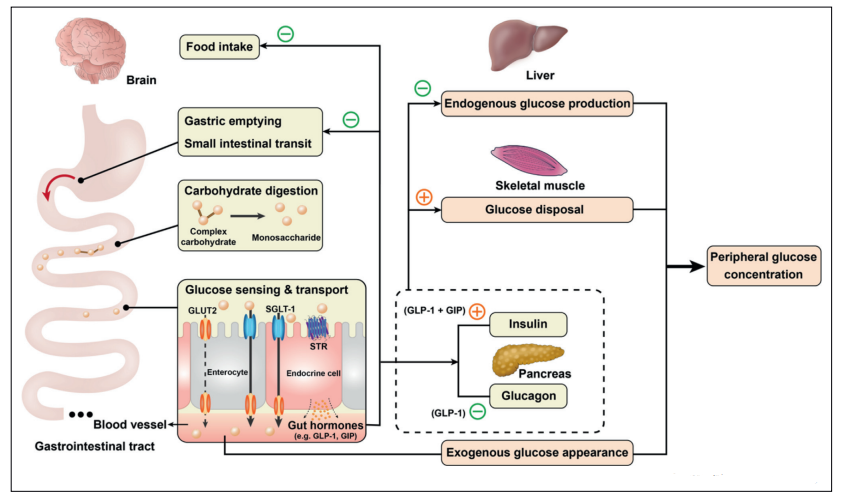
\includegraphics[width=14cm]{images/glucose_absorption.png}
\caption{Illustrartion of the glucose absorption process in the human body\cite{glucose_absorption}.}
\end{figure}

\subsection{Interstitial glucose}
The bloodstream is not the only place where glucose is abundant. Interstitial glucose is a result of diffusion across the capillary 
barrier caused by a difference in glucose concentration between blood capillaries and the interstitial fluid between cells\cite{rebrin_can_2000}. Interstitial glucose can be utilized 
directly by tissues including fat and muscle cells\cite{interstitial_glucose}. 

The time it takes for glucose to diffuse over the capillary barrier results in a lag time between changes in plasma glucose and interstitial
glucose. Apart from the lag time interstitial glucose behaves almost exactly the same as plasma glucose\cite{cengiz_tale_2009}. Figure 2 illustrates the diffusion of 
glucose molecules over the capillary barrier between the blood plasma (C1) and the interstitial fluid (C2). A CGM sensor is able to utilize interstitial glucose to measure plasma glucose. 


\begin{figure}[H]
\centering
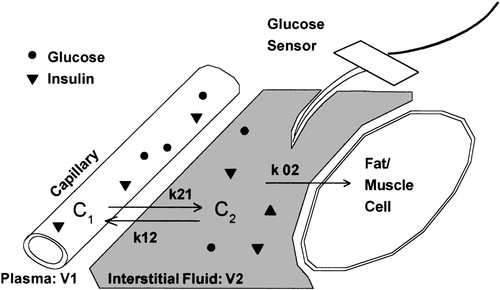
\includegraphics[width=14cm]{images/interstitial_glucose.jpeg}
\caption{Interstitial glucose as a result of diffusion over the capillary barrier\cite{interstitial_glucose}.}
\end{figure}

\subsection{Fasting Plasma Glucose}
Fasting plasma glucose (FPG) is a metric used when evaluating the metabolic health of an individual\cite{the_expert_committee_on_the_diagnosis_and_classification_of_diabetes_mellitus_report_1997}\cite{ekoe_screening_2018}. An FPG test is usually 
measured from a blood sample taken during a medical appointment. An FPG test measures the plasma glucose
concentration in the bloodstream. FPG is measured in the units mmol/L or mg/dL. This thesis uses the unit mmol/L.

A clinical FPG test requires an 8-hour fasting window. Fasting is defined as no caloric intake during a certain time 
period\cite{the_expert_committee_on_the_diagnosis_and_classification_of_diabetes_mellitus_report_1997}.
During the fasting widow, the patient is not allowed to eat or drink anything except water. This 
is to ensure that blood glucose levels have time to settle and are not affected by earlier nutritional 
intake. 

Every meal generates a corresponding spike in blood glucose. The size of the spike
depends on the nutritional content of the meal\cite{pi-sunyer_glycemic_2002}. Figure 3 illustrates how nutrition causes an elevation in 
blood glucose that settles over time as long as no more food is ingested. The data presented in Figure 3 is acquired from the data set provided by Veri.

\begin{figure}[H]
\centering
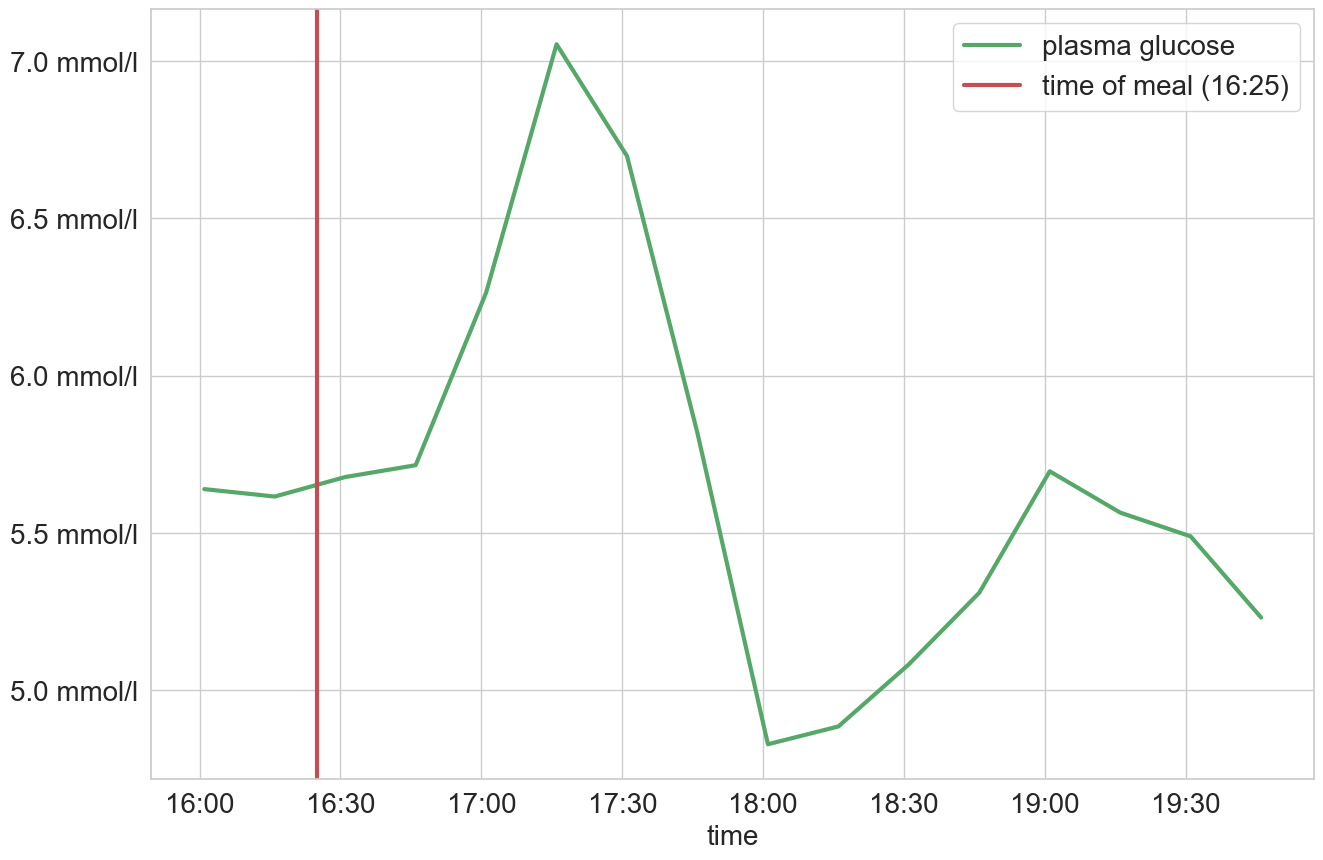
\includegraphics[width=14cm]{images/after_meal_glucose.png}
\caption{Elevation in blood glucose caused by nutritional intake. The data presented in this figure is acquired from the data set provided by Veri.}
\end{figure}

Studies have shown that the traditional 8-hour fasting window may not be necessary for the human body
to reach FPG levels\cite{moebus_impact_2011}. According to \cite{moebus_impact_2011}, a
fasting window of 3 hours is enough to achieve a reliable fasting plasma glucose measurement. The data presented
in \cite{moebus_impact_2011} is enough to challenge the traditional approach of an 8-hour fasting window but further 
research is required to establish the 3-hour fasting window as a clinical method. 
 
A shorter fasting window is highly relevant when considering CGM as a method for approximating FPG. CGM data 
doesn't always ensure that the patient has fasted for at least 8 hours. As a matter of fact, an 8-hour fasting window 
rarely happens during waking hours. With a shorter fasting window, a larger portion of the CGM data could be utilized
without having to be restricted to longer fasting periods. 

FPG is a recommended screening method when evaluating the risk of developing type 2 diabetes\cite{ekoe_screening_2018}.
Normal FPG levels range between 4.0 mmol/L and 5.6 mmol/L. An FPG value of 5.6 - 6.0 mmol/L 
indicates a risk of developing type 2 diabetes\cite{mathew_blood_2022}. Here it is worth mentioning that a 
momentary elevated FPG value is not necessarily a problem. Nevertheless, elevated FPG levels 
over a longer period of time are a strong indicator of metabolic abnormalities. 

Prediabetes is a state in which FPG levels exceed normal levels to reach values of 6.1 - 6.9 mmol/L. 
An FPG value of 7 mmol/L is diagnosed as diabetes\cite{diabetes_tests}.
If FPG levels stay in the abnormal range without exceeding 7 mmol/L the patient should continue frequent 
screening and apply lifestyle changes to ensure that FPG levels are kept under control\cite{ekoe_screening_2018}.

\subsection{Impaired Fasting Glucose and Impaired Glucose Tolerance}
Type 2 diabetes develops over a longer period of time. Impaired glucose tolerance (IGT) and impaired fasting
glucose (IFG) are both complications associated with the early stages of type 2 diabetes\cite{walker_diet_2010}.
IFG is defined by the FPG value of a patient. A patient with an elevated FPG value of 5.6-7 mmol/L is diagnosed 
with IFG \cite{nathan_impaired_2007}. IGT is determined by an Oral glucose tolerance 
test (OGTT) together with an FPG test. 

An OGTT usually involves consuming a 75g glucose load, usually in the form of a concentrated 
glucose solution. Plasma glucose is measured 2h after consuming the concentrated glucose solution to achieve an OGGT value. 
A patient with an OGTT value of 7.8-11.1 mmol/L and an FPG value of < 7 mmol/L is diagnosed with IGT\cite{nathan_impaired_2007}. 
Here, an FPG value of > 7 mmol/L and an OGTT value of > 11.1 mmol/L strongly indicate that the patient has developed type 2 
diabetes\cite{walker_diet_2010}\cite{diabetes_tests}.

The overlap in FPG shows that one can suffer from both IFG and IGT. Historical patterns show that among individuals 
diagnosed with either IGT or IFG, 25\% progress to diabetes, 50\% remain in the abnormal range 
without developing diabetes, and 25\% reacquire normal glucose tolerance. 
Being diagnosed with both of these metabolic complications doubles the probability of developing diabetes\cite{nathan_impaired_2007}.


\subsection{Correlations between lifestyle and blood glucose}
Diet, sleep, exercise, and stress all affect FPG. A healthy lifestyle 
includes favorable management of all four subcategories. Failing to control these may result in 
unhealthy fluctuations in FPG leading to metabolic disorders including IGT, IFG, and eventually, type 2 diabetes\cite{yamaoka_effects_2012}.

The earlier a patient detects FPG abnormalities, the better. 
Metabolic disorders usually develop over a longer period of time. A healthy lifestyle can not only prevent but also 
reverse metabolic complications, especially if caught in the early stages\cite{taylor_type_2013}. 

\subsubsection{Sleep}
The natural fasting window during sleeping hours allows for blood glucose to settle and reach FPG levels. A good night's sleep often results in a 
fasting window of at least 8 hours, fulfilling the traditional requirements of fasting plasma glucose.

A long night's sleep is not always favorable when it comes to FPG. Studies 
have shown an association between elevated FPG levels and sleep duration. A sleeping duration of under 6 hours or over 8 hours
has been shown to cause elevated FPG levels\cite{nakajima_association_2008}. 


\subsubsection{Diet}
Diet has a major impact on plasma glucose concentration\cite{russell_impact_2016}. Food is the main 
source of nutrition in the human body. During digestion, carbohydrates break down into glucose. 
Glucose is then absorbed into the bloodstream by the small intestine, as explained in Chapter 2.1, 
for the body to use as energy or store for later use. 

Carbon hydrates can be divided into simple and complex carbohydrates\cite{griel_changing_2006}. 
A simple carbohydrate is either a monosaccharide or a disaccharide.
The simple chemical structure of simple carbohydrates allows the body to quickly
digest and utilize them for energy. As a result, simple carbon hydrates often cause a rapid 
elevation in plasma glucose concentration and insulin secretion\cite{holesh_carbs}.
Complex carbohydrates, on the other hand, are composed of three or more sugars chained 
together. Complex carbohydrates often contain fiber, vitamins, and minerals. As complex 
carbohydrates take longer to digest, they have less of an immediate impact on plasma glucose\cite{holesh_carbs}.
Most foods contain both simple and complex carbohydrates but one is usually more present\cite{russell_impact_2016}.

Table 1 concertizes simple and complex carbon hydrates with examples of sugars that fall into the two categories. Examples of food sources from where the different sugars can be obtained are also included. 

\begin{table}[H]
\begin{center}
\begin{tabular}{ | m{3cm} | m{4cm}| m{4cm} | }
    \hline
    \textbf{carbohydrate} & \textbf{sugars} & \textbf{food sources} \\ 
    \hline
    & fructose & candy \\
    simple & lactose &  carbonated beverages \\
    & glucose & fruit juice \\
    \hline
    & cellobiose & broccoli \\
    complex & rutinulose & lentils \\ 
    & amylose & brown rice \\
    \hline
\end{tabular}
\caption{Examples of simple and complex carbohydrates in food\cite{physiology_carbohydrate}.}
\end{center}
\end{table}

The glycemic index is a way of ranking carbon hydrates based on how they affect plasma glucose.
On a scale of 0-100, foods rated >70 are considered high glycemic foods. Medium-level foods
are rated 56-69 and low-glycemic 55 or less\cite{atkinson_gi}. Glucose has a glycemic index of 
100 and is considered a reference point for the top of the scale.

The higher the glycemic index the higher the fluctuations in plasma glucose\cite{pi-sunyer_glycemic_2002}. Studies have 
shown that eating large quantities of high-glycemic foods over a longer period of time 
has a negative effect on fasting plasma glucose and increases the risk of obesity, type 
2 diabetes, and heart disease\cite{pi-sunyer_glycemic_2002}. Table 2 presents examples of foods and their corresponding 
glycemic index.

\begin{table}[H]
\begin{center}
\begin{tabular}{ | m{5cm} | m{2cm} | }
    \hline
    \textbf{food} & \textbf{GI} \\ 
    \hline
    apple, raw & 36 $\pm$ 2\\
    milk, full fat & 39 $\pm$ 3 \\
    porridge & 55 $\pm$ 2 \\
    potato, boiled & 78 $\pm$ 4 \\
    white table sugar, glucose & 100 \\
    \hline
\end{tabular}
\caption{Average GI of common food sources\cite{gi_indexes}.}
\end{center}
\end{table}

\subsubsection{Exercise}
Exercise has been proven to cause both elevations and dips in plasma glucose depending on
the type of workout. During high-intensity workouts such as heavy weightlifting and sprints, 
the body produces adrenaline. 
Adrenaline stimulates the liver to release glucose causing 
rapid elevation in plasma glucose\cite{excersise_glucose}. Aerobic exercise on the other hand
will lower your glucose levels during the workout. During moderate exercise, the muscles use more glucose than the body releases causing 
lower blood glucose levels.
Studies have also shown that regular aerobic 
exercise can lower FPG and 2-h postprandial blood glucose levels in diabetic patients\cite{shahgholian_effects_2015}.  

\subsubsection{Stress}
Stressful situations such as infections, serious illnesses, or significant emotional stress
cause insulin levels to fall and the body to produce adrenaline. As a result, stress 
stimulates the liver to release glucose causing elevations in plasma glucose\cite{stress_glucose}. 
Studies have shown that stress has a negative impact on FPG and may lead to diabetes-related
morbidities\cite{yitshak-sade_association_2020}.

\subsubsection{Obesity and type 2 diabetes}
The prevalence of obesity is one of today's most eminent health problems across the globe\cite{chooi_epidemiology_2019}. 
Obesity is a result of an unhealthy lifestyle over a longer period of time. A patient with a BMI of 30 or higher
is diagnosed with obesity \cite{jequer_pathways}. If not treated correctly, obesity 
leads to elevations in FPG causing IGT, IFG, and eventually diabetes\cite{garber_obesity_2012}. 

Studies have shown that correctly implemented lifestyle changes in obese individuals and patients 
diagnosed with prediabetes can lower FPG levels and reduce the risk for type 2 diabetes 
significantly\cite{taylor_type_2013}\cite{walker_diet_2010}. Other studies have also shown 
how type 2 diabetes can be reversed by diet\cite{taylor_type_2013}. A strict low-calorie diet
has been proven to bring FPG to normal levels among individuals diagnosed with type 2 diabetes\cite{taylor_type_2013}. 

\subsection{Continuous Glucose Monitoring}
The first CGM device was approved in 1999 by the U.S. Food and Drug Administration. Since then, 
technology has improved significantly and CGM has established itself as a viable alternative to 
glucose monitoring and management\cite{garg_new_2018}. 

Today, CGM is not only able to monitor glucose levels 
but it can also be paired with an insulin pump to automate insulin dosage in diabetes patients\cite{vettoretti_combining_2019}. 
There are two components in a CGM device, an electrochemical sensor implanted in the subcutaneous 
tissue of the abdomen or the arm or the stomach, and a monitor displaying glucose data\cite{vettoretti_combining_2019}. 
Today, the monitoring part of CGM is often handled by a mobile application. These mobile applications have developed to 
become useful tools for helping people with their glycemic control. Aboot's LibreLink application, for example, 
comes with additional features of an alarm that alerts the user when blood glucose reaches an unhealthy level\cite{librelink}. 

All the data used in this thesis is obtained by a CGM form known as flash glucose monitoring.
Flash glucose monitoring is based on CGM technology and offers lower daily costs and does not require regular calibration.
A flash glucose monitoring device requires scanning the sensor at least every 8 hours to access 
full 24-hour data\cite{petrie_improving_2017}. 

Veri utilizes flash glucose monitoring by pairing its application with the Freestyle Libre sensor by Abbot. Utilizing Abbot's LibreLink
application Veri's users are able to scan their Freestyle Libre sensor to access 24-hour glucose data. 
Veri's application continuously fetches glucose data from LibreLink for analysis. The data set used in this 
thesis is obtained by the combination of the Freestyle Libre sensor, the LibreLink application, and Veri's own application.


\subsubsection{Flash glucose monitoring sensor}
CGM measures interstitial glucose, found in the interstitial fluid between cells. 
The in-vivo sensor, which utilizes a small filament to measure glucose, is inserted under the skin with the help of a needle. 
The filament of the CGM sensor contains an enzyme known as glucose oxidase and is made up of a three-electrode system\cite{schmelzeisen-redeker_overview_2013}. 

When inserted through the skin, the enzyme reacts with the interstitial fluid resulting in the oxidation of hydrogen peroxide. 
This process generates an electrical current that is indicative of the glucose concentration\cite{schmelzeisen-redeker_overview_2013}.
Figure 4 presents a visual comparison of the physiological differences between the traditional approach to glucose monitoring and flash 
glucose monitoring. 

\begin{figure}[H]
\centering
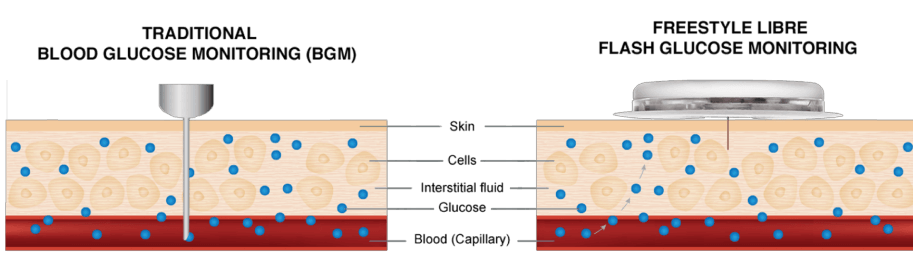
\includegraphics[width=15cm]{images/cgm.png}
\caption{Visual comparison of the physiology behind the traditional approach to blood glucose monitoring and flash glucose monitoring\cite{freestyle_cgm}. Compared to a traditional blood sample, the CGM sensor utilizes a small filament containing an enzyme named glucose oxidase. Glucose oxidase reacts with the 
interstitial fluid producing an electrical current that is indicative of the glucose concentration.}
\end{figure}

\subsubsection{Limitations}
Despite its popularity, CGM has its limitations. The in vivo response to a needle-type biosensor has
been one of the biggest challenges to accurate CGM measurements. The infiltration
of proteins, the release of cytokines and reactive oxygen species, and subsequent
influx of inflammatory cells all contribute to the instability of implanted glucose sensors\cite{gifford_cgm}. 

When measuring interstitial glucose it is important to consider how it differs from blood glucose. As mentioned, interstitial 
glucose is the result of diffusion between blood capillaries and the interstitial fluid. The lag time caused by 
the time it takes for glucose to diffuse over the capillary barrier
causes delay between interstitial glucose and plasma glucose. Studies have also shown that 
distortions may occur when comparing interstitial glucose measurements to plasma glucose\cite{cobelli_interstitial_2016}. 

Another drawback of the CGM device is its seemingly short lifetime. For hygienic reasons, the sensor of a CGM device has to be replaced every 10-14 days.
A process that may be perceived as disruptive and unwieldy.

\subsection{FPG monitoring as a preventive measure for disease}
The prevalence of obesity and type 2 diabetes is closely related to FPG. Obesity is a result of an unhealthy lifestyle over a longer period of time,
causing elevated FPG levels\cite{garber_obesity_2012}. Elevated FPG levels over a long period of time lead to complications including IFG 
and IGT that ultimately may develop into type 2 diabetes. Patients diagnosed with IFG and IGT run a significant risk of developing type 2 diabetes\cite{nathan_impaired_2007}. 

As discussed in Chapter 2.2, IFG and IGT are both defined using FPG. With frequent FPG tests, patients are able to detect
elevations in FPG and seek care before FPG reaches unhealthy levels. Optimally, FPG abnormalities are detected and remedied before they develop into IFG or
IGT. Proactive lifestyle changes during the prediabetes stage can prevent IFG, IGT, and the development of type 2 diabetes\cite{taylor_type_2013}. 
%% END TEXT %%
\clearpage

%%%%%%%%%%%%%%%%%%%%%%%
%% RESEARCH MATERIAL %%
%%%%%%%%%%%%%%%%%%%%%%%%
\section{Research material}
%% TEXT %%
This chapter summarizes the research material used in this thesis. In this thesis, the data set provided by Veri was used to illustrate trends in blood glucose.
The graphical demonstrations presented in this thesis help the reader visualize how blood glucose is affected by lifestyle and how FPG can be approximated by CGM data.

\subsection{Data set}
The data set used in this thesis contains deidentified user health data obtained by Veri. The data set includes 
glucose data from roughly 6000 Veri users. Apart from glucose data, the data set also includes the users' sleep,
exercise, and demographic information. 

As Veri's data depends on user input the data set is incomplete to some extent. Non-logged events, 
absent profile information, and irregular glucose scans result in missing glucose data. Nevertheless, 
the data set provides an adequate overview of the glucose data among the users.

Figure 5 presents a graphical summary of the demographic data of the data set. The height distribution of the users 
is normally distributed between 140-200cm with a mean of 171.1cm. The weight distribution of the users 
follows a slightly skewed normal distribution between 40-150kg with a mean of 79.4kg. The height and length
distributions result in an average BMI of just under 25kg/\si{\meter\squared}. Among the users, 
3400 identify as female, 2100 as male.


% PICTURE: demographics
\begin{figure}[H]
\centering
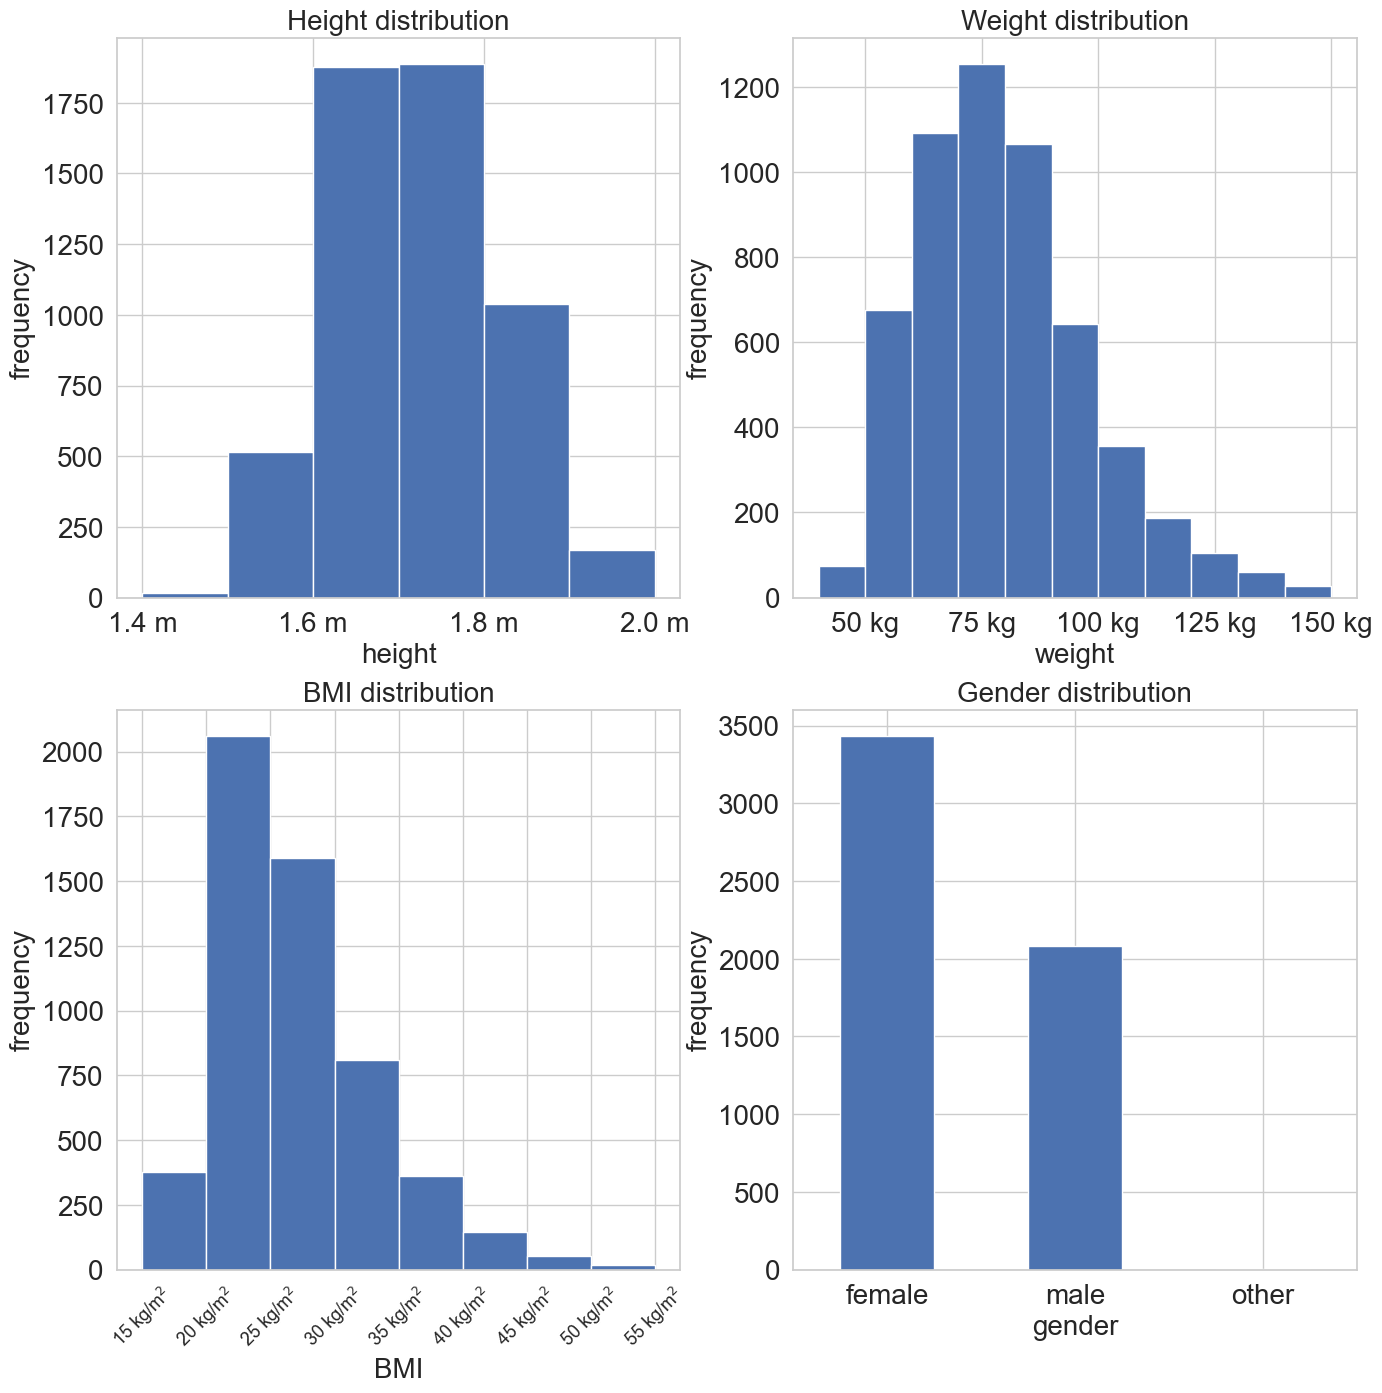
\includegraphics[width=14cm]{demographics.png}
\caption{Graphical summary of the demographics of the data set used in this thesis to visually demonstrate how FPG can be approximated from CGM data.}
\end{figure}

The data set also contains user event data, including sleep, meal, 
and exercise information. The event data visualizes the habits of the users.   
Figure 6 shows a graphical summary of the sleep and meal information of the users. 

The first histogram shows the users' preferred number of meals per day. The majority of the users prefer 3 meals a day.
Studies have shown that the number of meals per day has an impact on blood glucose, where a larger number of meals 
result in augmented glucose levels throughout the day\cite{HOLMSTRUP2010e277}.

The second histogram visualizes the distribution of the duration of every recorded sleeping event in the data set.
As shown in the histogram. Most users sleep between 7 and 9 hours. The sleeping patterns of the users
are highly relevant to the topic of finding FPG through CGM. A good night's sleep of over 8 hours automatically fulfills the 
fasting window requirement of FPG. Unfortunately, this is not always the case as the histogram 
implies.


% PICTURE: events
\begin{figure}[H]
\centering
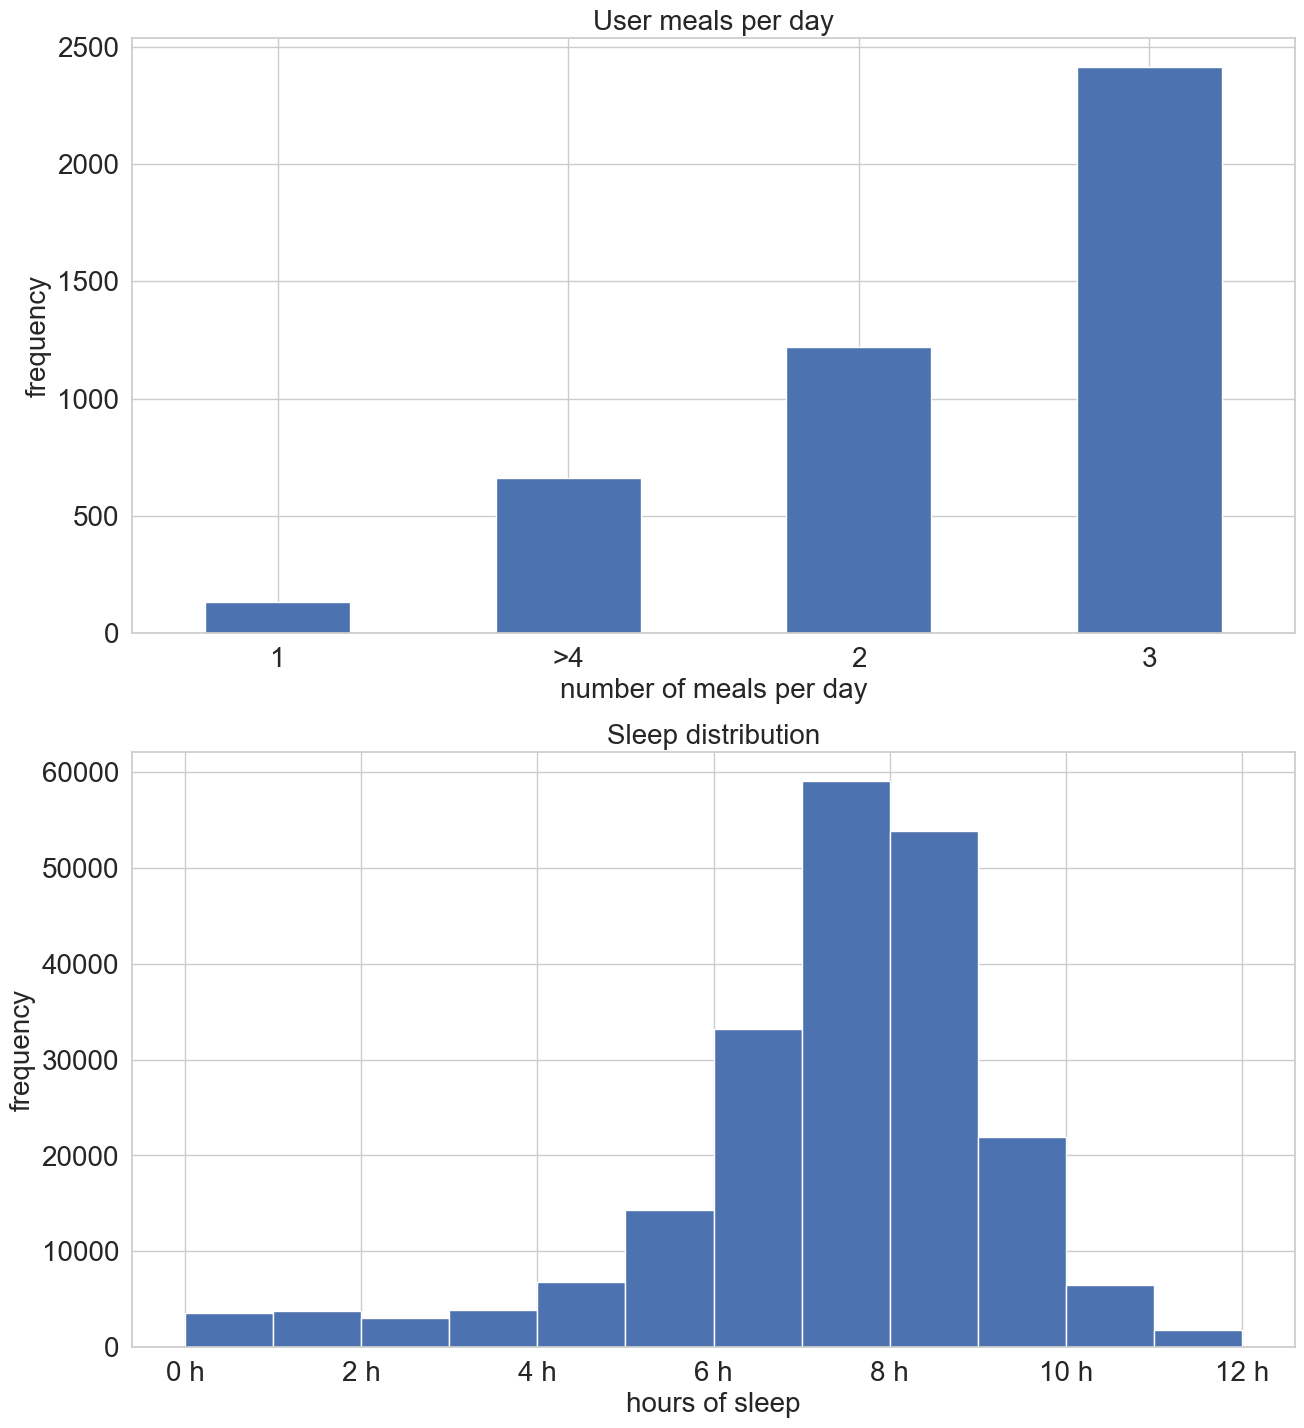
\includegraphics[width=14cm]{events.png}
\caption{Graphical summary of user event data obtained from the data set provided by Veri.}
\end{figure}

Every user has their own set of glucose values fetched by a CGM device. Each glucose value is paired with a timestamp. 
Below is a histogram illustrating the mean glucose values of Veri's users. The average mean glucose of the users is 5.45 mmol/L with
a standard deviation of 0.57 mmol/L. As \cite{mathew_blood_2022} states, normal FPG levels range between 4.0 mmol/L and 5.6
mmol/L. The average glucose value of a user will be higher compared to the FPG value of the user as the average glucose value
includes meals and other events affecting blood glucose. Figure 7 shows the distribution of user mean glucose.

% PICTURES: glucose means
\begin{figure}[H]
\centering
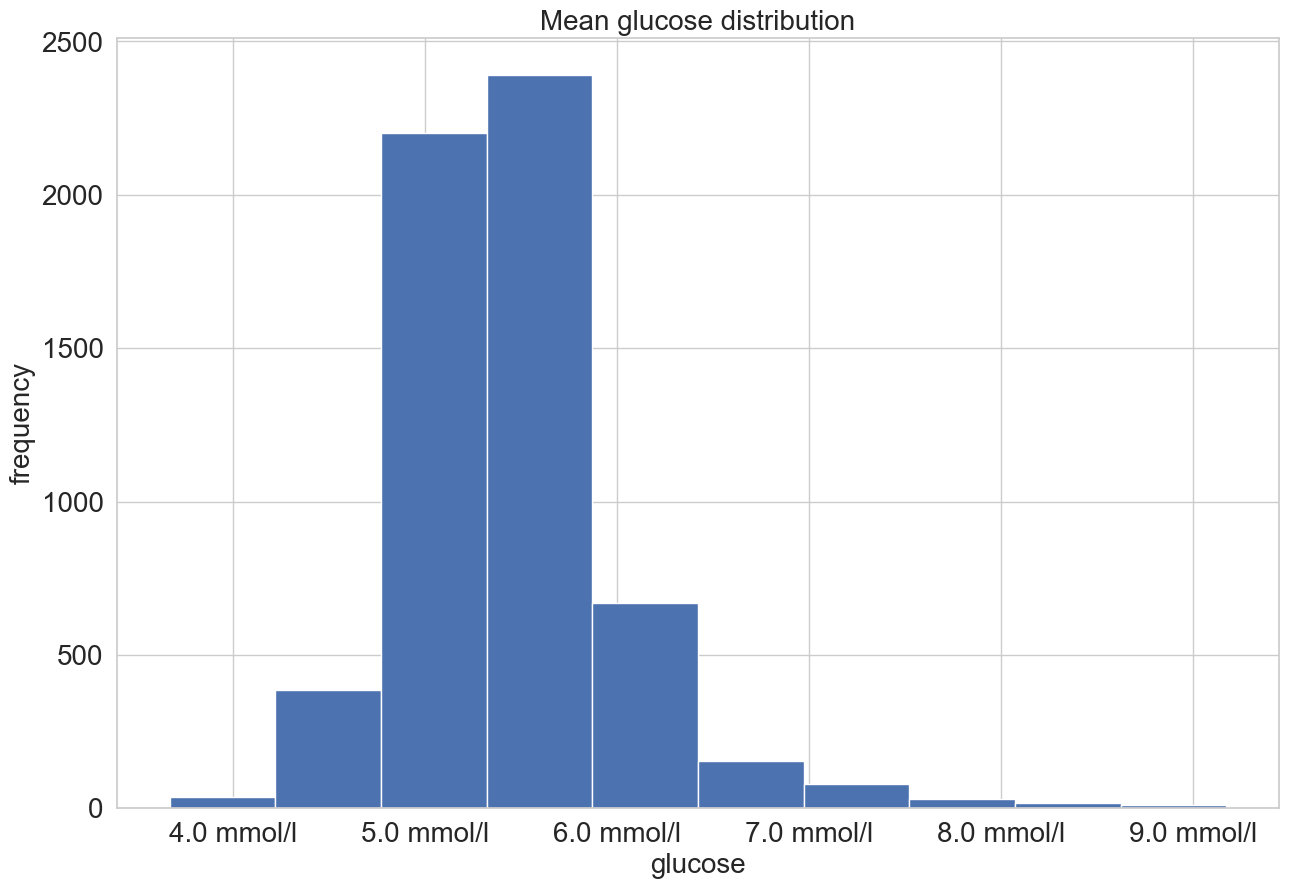
\includegraphics[width=14cm]{glucose_means.png}
\caption{Histogram visualizing user mean glucose distribution of the data set provided by Veri.}
\end{figure}

When looking at the glucose data on an individual level, lifestyle's impact on glucose is evident. Figure 8 shows a graphical visualization
of the glucose data of a single user over a period of two days. The glucose data used to visualize glucose trends is obtained from the data set presented in this chapter. During the daytime variation in blood glucose is high due to meals and other lifestyle-related events\cite{yamaoka_effects_2012}. During nighttime blood glucose has time to settle and reaches a more steady state due to the natural fasting window occurring\cite{sato_acute_2011}.

% PICTURE: user glucose
\begin{figure}[H]
\centering
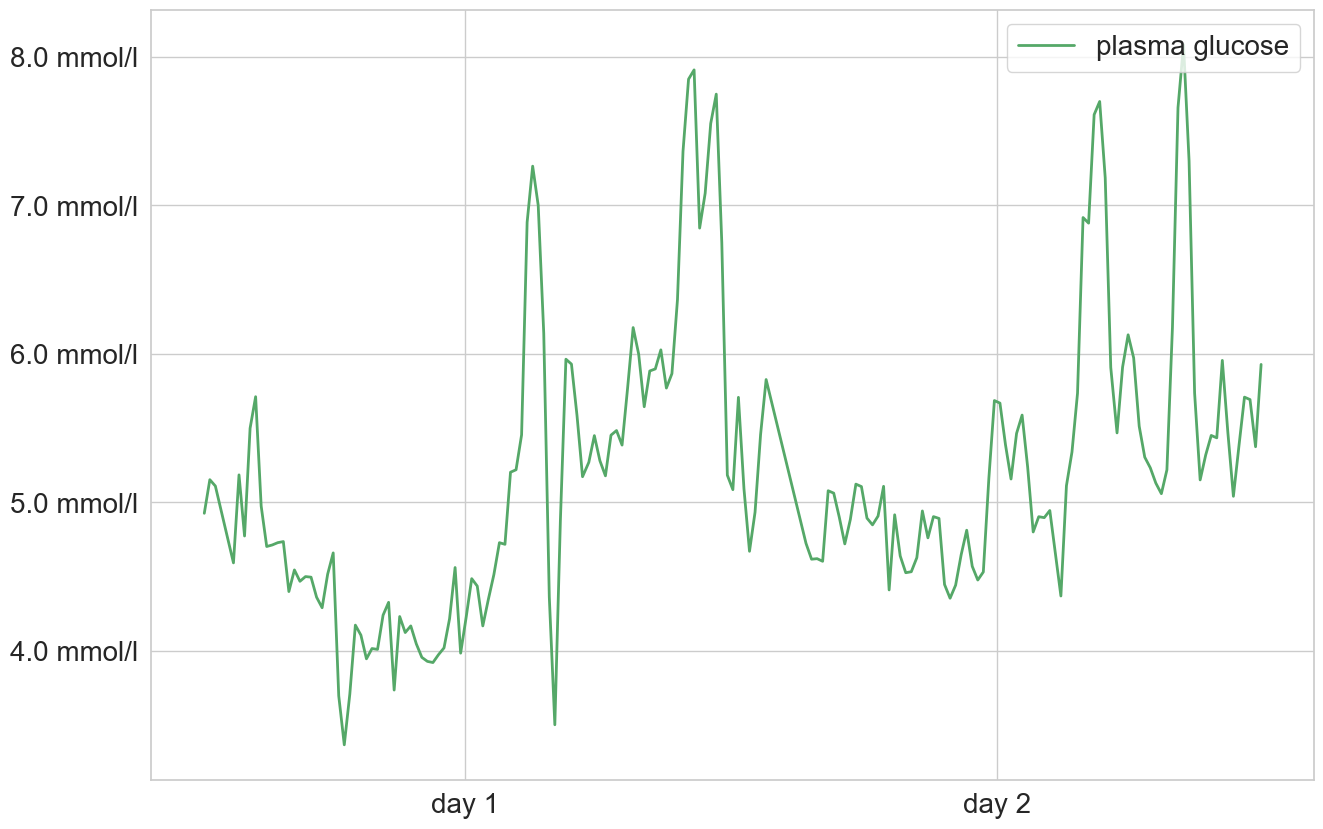
\includegraphics[width=14cm]{user_glucose.png}
\caption{Glucose curve of a single user obtained from the data set provided by Veri.}
\end{figure}

The glucose data alone provides an incomplete picture of lifestyle's impact on blood glucose. Figure 9 shows the same glucose 
data as in Figure 8 but with added overlays of the events occurring during the same time interval. The blue areas represent sleep and the 
red lines represent meals. 

The glucose data and the added events provide a more complete picture and explain the daily fluctuations in blood glucose. As the graph shows, 
the fluctuations in blood glucose during sleeping are much lower compared to the daytime. As mentioned, during sleeping 
hours, blood glucose usually has time to reach FPG levels due to the natural fasting window occurring. FPG levels may vary from night to night. As \cite{nakajima_association_2008} states, sleeping duration has an impact on FPG levels. Elevations in nightly FPG
may be caused by many different factors, and duration of sleep is one of them. 

Studies have shown that late evening meals result in elevated nocturnal blood glucose levels\cite{sato_acute_2011}. Glucose tolerance decreases during
the night. Late evening meals not only affect nocturnal glucose levels but may also generate larger glucose spikes than a normal evening meal\cite{sato_acute_2011}.

% PICTURE: user glucose + events
\begin{figure}[H]
\centering
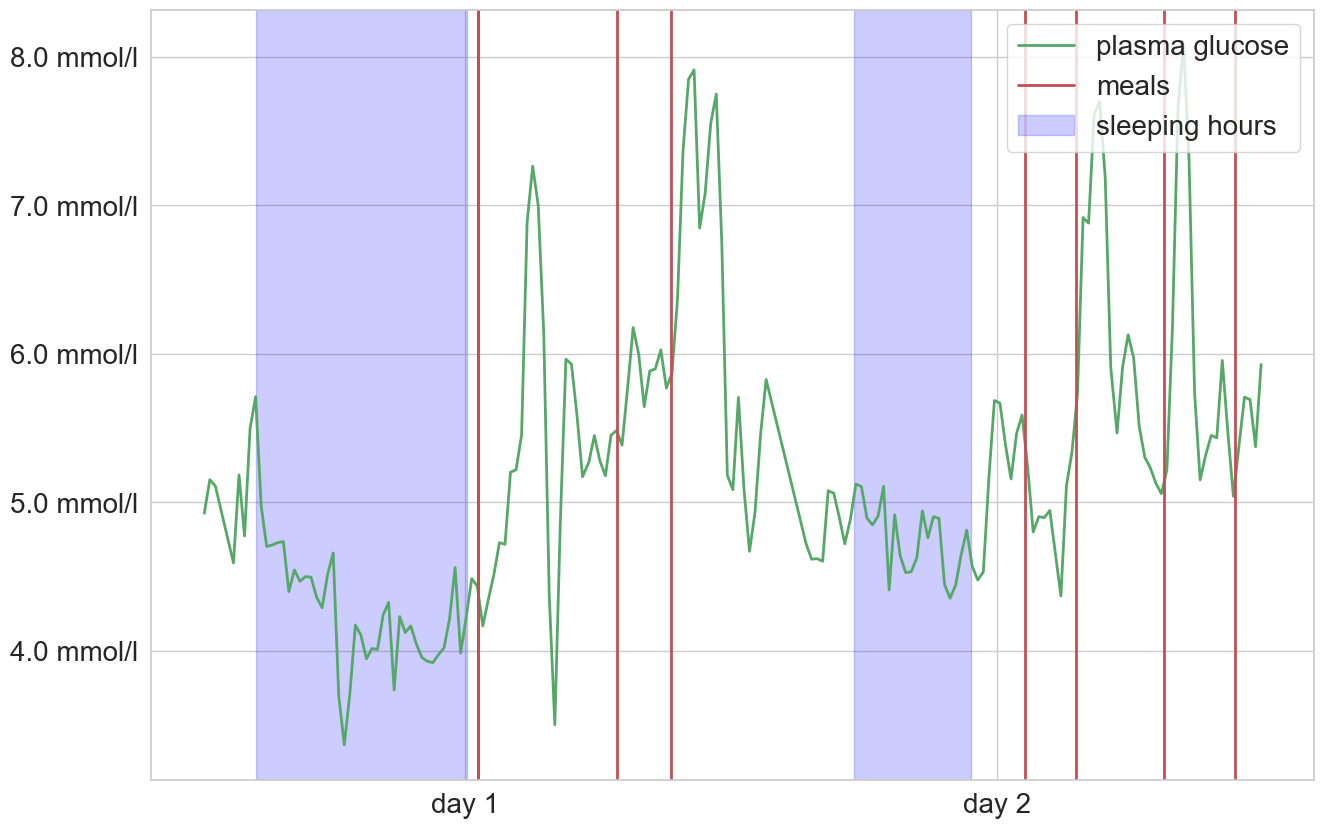
\includegraphics[width=14cm]{user_glucose_and_events.png}
\caption{Glucose data of a single user with additional events obtained from the data set provided by Veri.}
\end{figure}

\section{FPG approximations based on CGM data}
This chapter includes four visual demonstrations of FPG approximations assessed from CGM data.
The data presented in this chapter is obtained from the data set provided by Veri.
When approximating FPG from CGM data, a choice has to be made on whether to stick
with the traditional approach of an 8-hour fasting window\cite{mathew_blood_2022} or utilize a shorter fasting window\cite{moebus_impact_2011}.
A major flaw of the traditional 8-hour fasting window is that it limits the data by excluding a larger portion of the data. 8-hour fasting windows rarely occur outside
sleeping hours.

A 3-hour fasting window occurs more frequently, usually several times per day. Hence, a shorter fasting window could be utilized to obtain several FPG 
measures per day. This allows for a comparison of meals and how they affect FPG. The major drawback of a 3-hour fasting window approach is that it currently lacks
research supporting it. The data presented in \cite{moebus_impact_2011} challenges the 8-hour fasting window but further research has to be made
to establish the 3-hour fasting window as a clinical method for measuring FPG.

The baseline for determining FPG from CGM data would be to take a single glucose sample at the end of the determined fasting window. Let's start 
by considering a minimum fasting window of 8 hours\cite{mathew_blood_2022}. Figure 10 shows the same graph of glucose values 
and events as in Figure 9 with additional FPG measurements marked with black dotted lines. The FPG samples 
are taken after a fasting window of at least 8 hours. This momentary sample approach is equal to the traditional way of 
measuring FPG from a blood sample taken after an 8-hour fasting window, disregarding the MARD of the CGM device. 

Figure 10 depicts how this approach leads to identifying two FPG values - 4.01 mmol/L and 4.89 mmol/L. 
These measurements are already adequate approximations of FPG based on the requirements of a traditional FPG test\cite{mathew_blood_2022}.
However, the momentary samples fail to utilize the continuous stream of data provided by the CGM device.

% PICTURE: 
\begin{figure}[H]
\centering
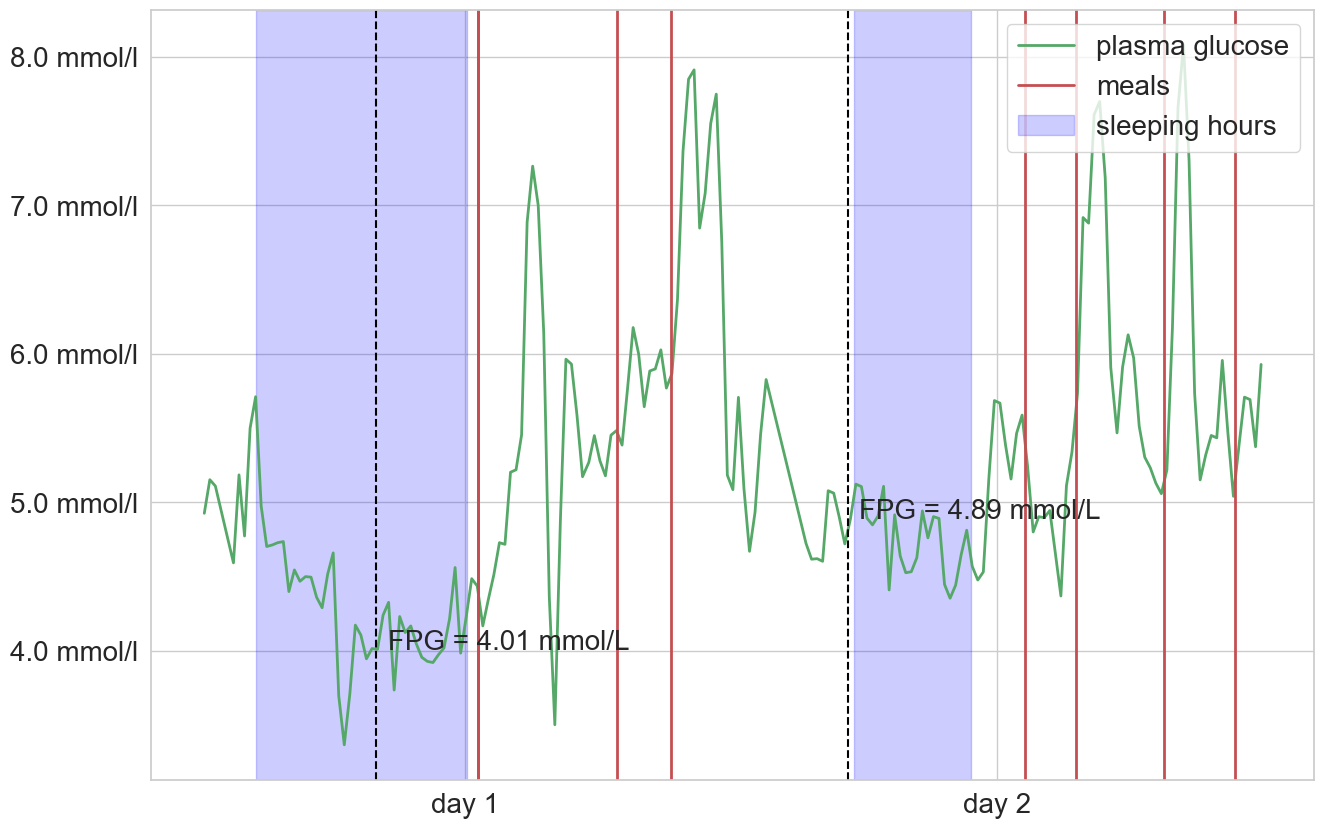
\includegraphics[width=14cm]{images/user_glucose_and_fpg1.png}
\caption{Individual FPG samples obtained after an 8-hour fasting window.}
\end{figure}


To fully utilize the continuous data stream of a CGM device an alternative would be to include all glucose data between 
the point of fulfilling the fasting window requirement and the next meal. FPG requires a fasting window of a certain duration.
Hence, every glucose measurement between the end of said fasting window and the next nutritional intake cloud be considered an FPG value.

In Figure 11, the FPG approximation is achieved by calculating the mean value of the glucose data within the defined window. 
In this case, the green area represents the glucose data used to calculate the mean FPG value between fulfilling the 
8-hour fasting window requirement and the next meal. This approach generated two mean FPG values of 4.14 mmol/L and 4.89 mmol/L. 

Compared to the momentary sample approach shown in Figure 10, the mean FPG approach generates an approximation that relies on a larger portion of the data
provided. As the glucose curve implies, fluctuations in blood glucose are evident even during longer fasting windows. 
A momentary measurement is heavily dependent on fluctuations in plasma glucose and the MARD of the CGM device. 
By calculating the mean blood glucose value over a longer fasting period, the impact of momentary fluctuations is  excluded. 
Further research has to be made on whether the mean value is the best way of approximating FPG based on the data included. Nevertheless,
the mean value succeeds to deliver an approximation independent of momentary fluctuations among the FPG values included.

When comparing the mean FPG values in Figure 11 to the momentary FPG samples in Figure 10, the results are similar. Nevertheless, the mean FPG values 
in Figure 11 are based on a larger portion of data, arguably providing a more complete picture of FPG levels during corresponding fasting periods.  

% PICTURE: 
\begin{figure}[H]
\centering
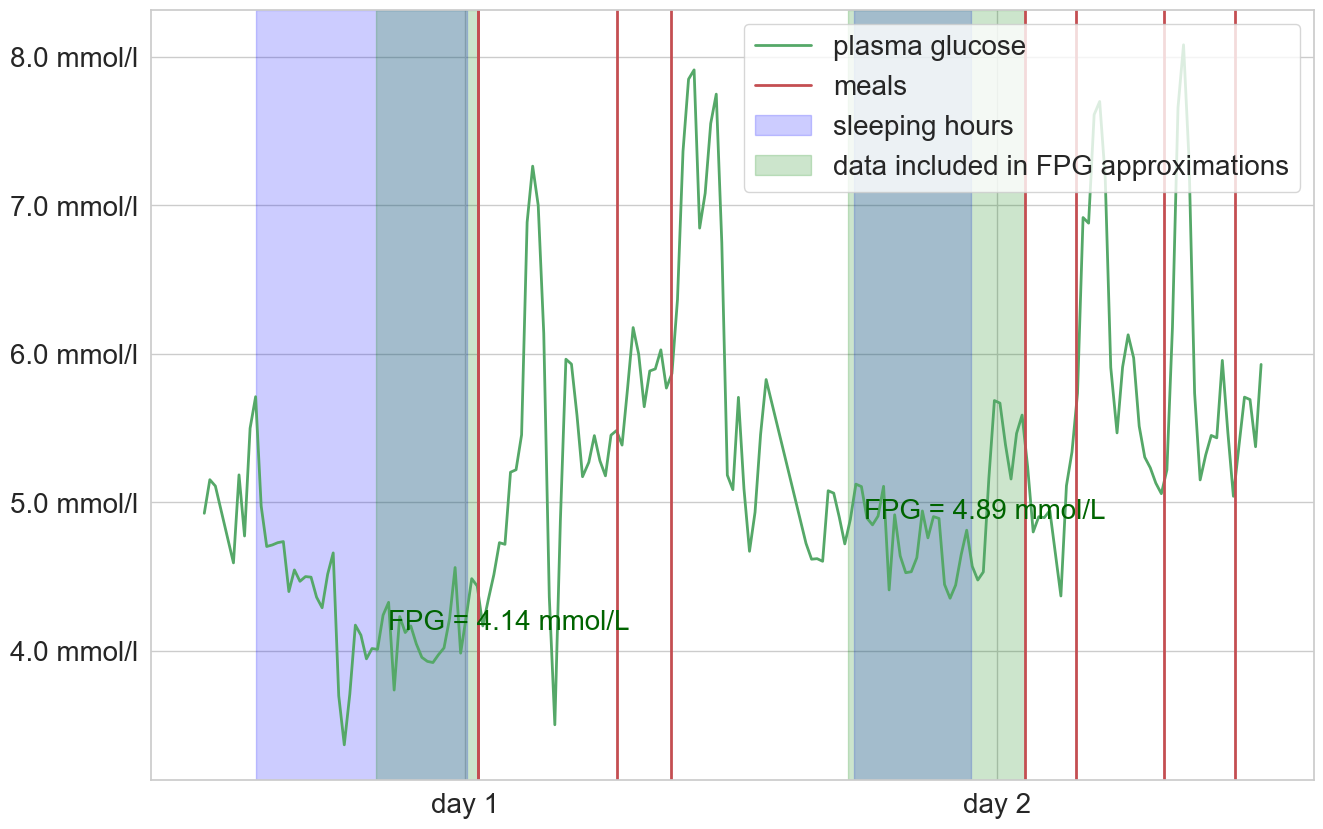
\includegraphics[width=14cm]{images/user_glucose_and_fpg2.png}
\caption{Mean FPG measurements with 8-hour fasting windows.}
\end{figure}

To include an even larger portion of the provided CGM data, a shorter fasting window of 3 hours can be utilized when approximating FPG\cite{moebus_impact_2011}. 
Firstly, the momentary sample approach is applied with a 3-hour fasting window. Figure 12 shows the glucose 
curve of the same individual with additional events and FPG measurements with a 3-hour fasting window. Compared to an 8-hour fasting window,
a 3-hour fasting window allows for 4 measurements instead of two in  this particular case. The momentary values measured were 4.70 mmol/L,
6.14 mmol/L, 5.70 mmol/L, and 5.31 mmol/L. A shorter fasting window usually generates a larger number of FPG measurements. 

As stated in Chapter 3.1, the majority of the users included in the data set eat 3 meals per day. 3 meals per day usually allow for multiple 3-hour fasting 
windows during the day. Nevertheless, there are also cases where a 3-hour fasting window generates an 
equal amount of FPG measurements as an 8-hour fasting window. 

In this particular case, when comparing the momentary samples of a 3-hour fasting window to the momentary FPG samples of an 8-hour fasting window, 
the 3-hour fasting window has 
a tendency of generating slightly higher values than an 8-hour fasting window. The difference is especially visible when looking at the second measurement in Figure 12. The momentary sample of 6.14 mmol/L is taken during the daytime between meals and is noticeably higher than both measurements in Figure 10.

% PICTURE: 
\begin{figure}[H]
\centering
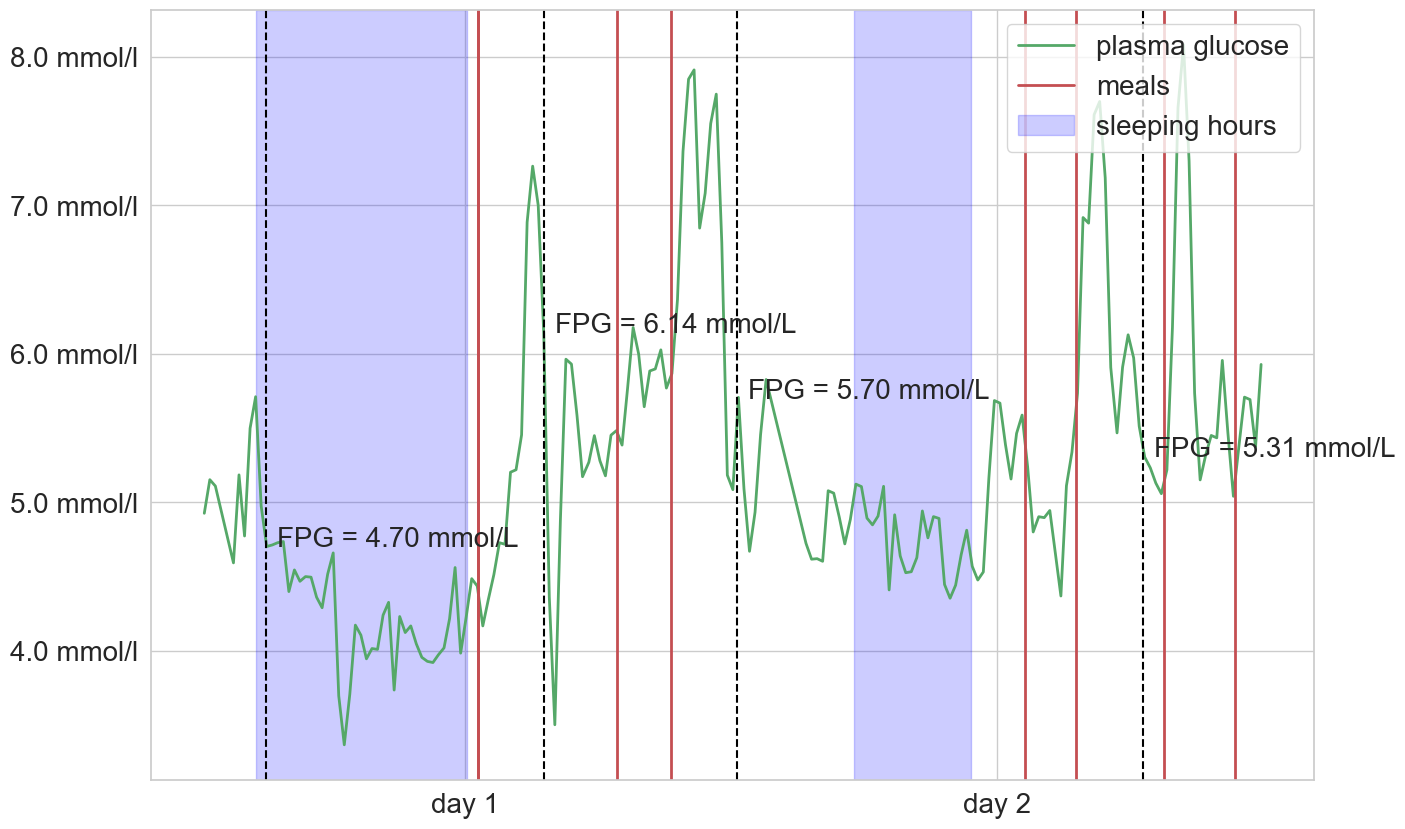
\includegraphics[width=14cm]{images/user_glucose_and_fpg3.png}
\caption{Individual FPG samples obtained after a 3-hour fasting window.}
\end{figure}

When applying the mean FPG approach to a 3-hour fasting window, the results in this particular case are noticeably lower. Figure 13 illustrates the data included between the 
end of the 3-hour fasting windows and their next corresponding meal. The mean FPG values measured in Figure 13 were 4.22 mmol/L, 5.17 mmol/L, 4.92 mmol/L, and 5.18 mmol/L. 
When comparing the values in Figure 13 to the values in Figure 12, the values in Figure 13 are noticeably lower. 

When comparing the mean FPG values generated by a 3-hour fasting window to the mean FPG value generated by an 8-hour fasting window, the trend is similar to
the comparison of the momentary FPG samples. The mean FPG values of 4.14 mmol/L and 4.89 mmol/L in Figure 11 correspond to the values of 4.22 mmol/l and 4.92 mmol/L in Figure 13. 
The 3-hour fasting window generates slightly higher mean FPG values than the 8-hour fasting window, indicating the need for further research to establish the 3-hour fasting window as a clinical method when measuring FPG\cite{moebus_impact_2011}.

% PICTURE: 
\begin{figure}[H]
\centering
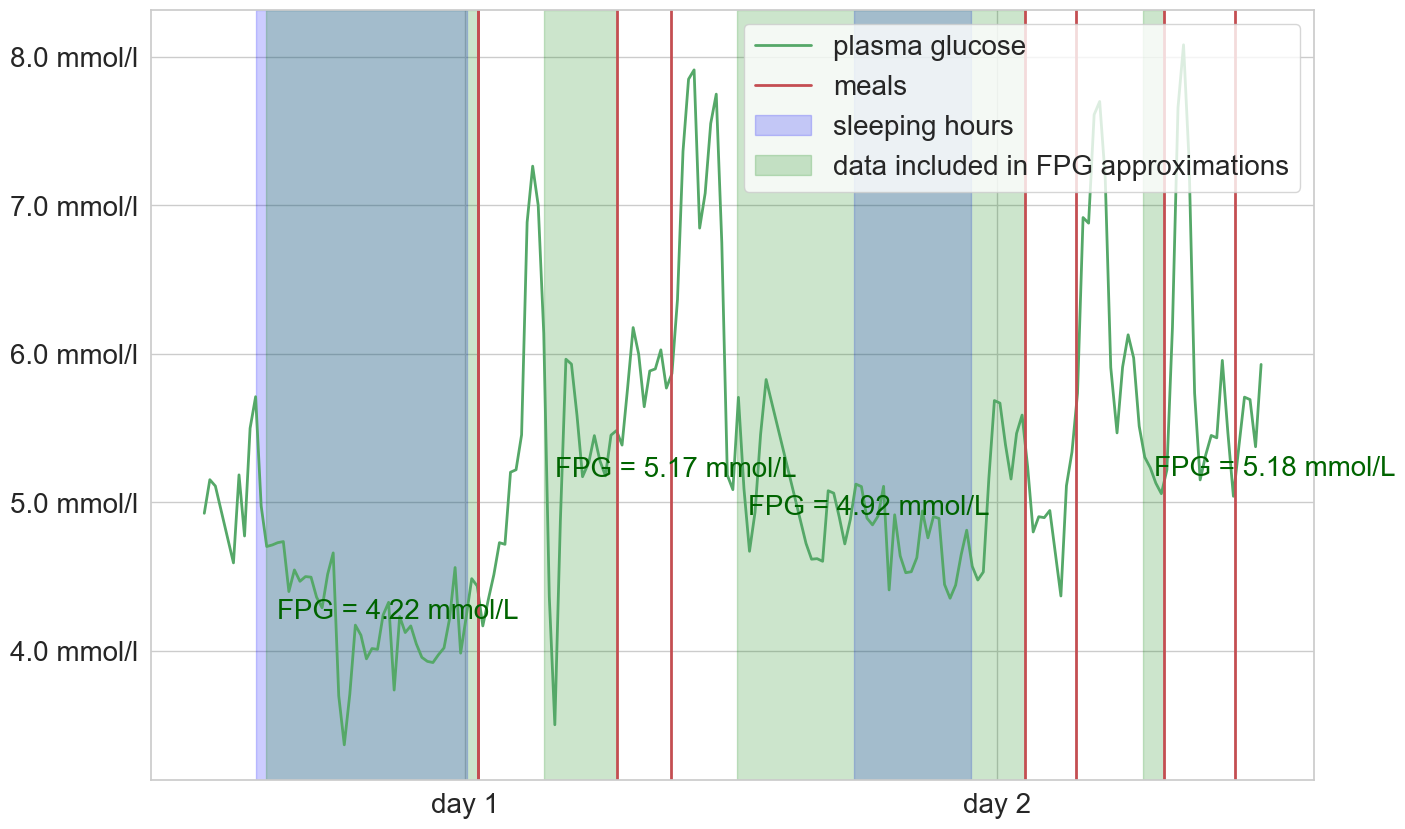
\includegraphics[width=14cm]{images/user_glucose_and_fpg4.png}
\caption{Mean FPG measurements with 3-hour fasting windows.}
\end{figure} 

To determine how the four methods of approximation presented in this chapter perform in general, further analysis would have to be performed on the data set. The data 
set includes glucose-related data from roughly 6000 users and allows for further research regarding the approximation of FPG from CGM data.
%% END TEXT %%
\clearpage


%%%%%%%%%%%%%%%%
%% Discussion %%
%%%%%%%%%%%%%%%%
\section{Discussion}
%% TEXT %%
An FPG measurement requires a fasting window of a debatable size. Traditionally, an 8-hour 
fasting window has been the clinical standard when measuring 
FPG\cite{the_expert_committee_on_the_diagnosis_and_classification_of_diabetes_mellitus_report_1997}. 
Newer research has challenged the traditional approach, stating that 8 hours of fasting may not be necessary to measure 
FPG\cite{moebus_impact_2011}. A shorter fasting window of 3 hours favors CGM-generated FPG approximations by  
allowing larger portions of the CGM data to be included in the approximation. Further research has to be done to
establish the 3-hour fasting window as a clinical method.

Possible methods for approximating FPG with CGM were illustrated in Chapter 4. Two different fasting window durations were applied.
The duration of the fasting windows applied were 8 hours\cite{the_expert_committee_on_the_diagnosis_and_classification_of_diabetes_mellitus_report_1997} 
and 3 hours\cite{moebus_impact_2011}. Firstly, similarly to the traditional approach of measuring FPG, 
momentary samples were taken from the CGM data at the end of each corresponding fasting window. The major flaw of the momentary sample 
approach is that it fails to utilize the continuous stream of data that a CGM device provides. Nevertheless, it corresponds to the 
traditional way of testing FPG through a single blood sample.

To include a larger portion of the data set, a mean FPG value was calculated using glucose data between the end of the 
previous fasting window and the next meal. The mean FPG approach allows approximations based on a much larger portion of 
the CGM data provided compared to the momentary sample approach. As FPG measurements require a certain fasting window, every 
glucose value obtained after the fasting window and before the next nutritional intake is classified as FPG.

When comparing the different methods in the particular case presented in Chapter 4, the 3-hour fasting 
window had a tendency to generate a slightly higher FPG value. The data presented in \cite{moebus_impact_2011} indicates that 
a fasting window under 8 hours generally generates a slightly higher FPG value than a fasting window over 8 hours.
These results imply that further research still has to be made for a 3-hour fasting window to be clinically approved\cite {moebus_impact_2011}.
The data presented in \cite{moebus_impact_2011} is still enough to challenge the traditional approach of an 8-hour fasting window when 
approximating FPG from CGM data.

Compared to the momentary sample approach, the mean FPG approach succeeds to utilize the full potential of the CGM device.
A momentary sample is similar to the traditional approach where FPG is measured from a blood sample. The major difference between a 
traditional FPG test and an FPG approximation obtained by a CGM device is 
the MARD of the CGM device\cite{rodbard_continuous_2016}. Today, the MARD of CGM is low enough to consider CGM as a valid method when 
approximating FPG\cite{rodbard_continuous_2016}.

When trying to achieve an FPG approximation based on a larger portion of the
CGM data, the average FPG approach is the more favorable method. Depending on the duration of the previous fasting window, the average 
FPG approach generates an approximation based on all glucose data between the end of the fasting window and the next meal. To include the maximum
amount of data in the approximation, a 3-hour fasting window would be the favored approach. The 8-hour fasting window is the safer approach
to ensure that the approximation is based on clinical research\cite{mathew_blood_2022}.
%% END TEXT %%
\clearpage


\section{Conclusion}
%% TEXT %%
FPG approximations from CGM data are made possible by obtaining meal-related information from the patient. Without knowing the time since the last nutritional intake of the patient it is hard to obtain a reliable FPG value. Wrongly approximated FPG values may lead to unnecessary worry and faulty diagnoses.


This thesis aimed to explore the possibility of using CGM data to approximate
FPG by comparing the traditional 8-hour fasting window to a shorter fasting window
of three hours. The result was obtained by combining earlier research with visual 
demonstrations of FPG approximations. The results still favor a longer fasting window of eight hours. Both earlier research and the visual demonstrations indicated that a shorter fasting window
of 3 hours has a tendency of generating slightly higher FPG approximations than a longer fasting window of at least 8 hours. Despite the difference being relatively small, further research still has to be made to establish a shorter fasting window as a clinical approach when approximating FPG
from CGM data.

Regular FPG approximations obtained by a CGM device do not require a medical appointment. 
By regularly monitoring FPG values, patients are able to react to elevations and apply lifestyle changes proactively to avoid further complications. Used correctly, FPG assessed by CGM favors 
metabolic health development. 
%% END TEXT %%
\clearpage

%%%%%%%%%%%%%%%%
%% REFERENCES %%
%%%%%%%%%%%%%%%%
\bibliographystyle{IEEEtran}
\bibliography{ref}
\clearpage

%% ADD POSSIBLE APPENDIX HERE
%% \thesisappendix

\end{document}
